

\documentclass{article}
\usepackage{amsmath}
\usepackage[utf8]{inputenc}
\usepackage{authblk}
\usepackage{setspace}
\usepackage[margin=1.25in]{geometry}
\usepackage{graphicx}
\graphicspath{ {./Images/} }
\usepackage{subcaption}
\usepackage{amsmath}
\usepackage{lineno}
\usepackage{wrapfig}
\usepackage{array}
\usepackage[section]{placeins}
\linenumbers

%%%%%% Bibliography %%%%%%
% Replace "sample" in the \addbibresource line below with the name of your .bib file.
\usepackage[
  backend=biber,
  bibencoding=utf8,
  style=nejm, 
  citestyle=numeric-comp,
  sorting=none]{biblatex}

\addbibresource{NMSunscreenBibTeX.bib}
%\addbibresource{reducedSunscreen}

 
%%%%%% Title %%%%%%
% Full titles can be a maximum of 100 characters, including spaces. 
% Title Format: Use title case, capitalizing the first letter of each word, except for certain small words, such as articles and short prepositions
\title{Investigating the Impact of Concentration on Non-Nano Zinc Oxide as a Viable Sun Protector: A Comparative Analysis with Commercial Sunscreens}

%%%%%% Authors %%%%%%
% Authors should be listed in order of contribution to the paper, by first name, then middle initial (if any), followed by last name.
% Authors should be listed in the order in which they will appear in the published version if the manuscript is accepted. 
% Use an asterisk (*) to identify the corresponding author, and be sure to include that person’s e-mail address. Use symbols (in this order: †, ‡, §, ||, ¶, #, ††, ‡‡, etc.) for author notes, such as present addresses, “These authors contributed equally to this work” notations, and similar information.
% You can include group authors, but please include a list of the actual authors (the group members) in the Supplementary Materials.
\author[1$\dag$]{Natalia C. Marquez}
\author[2$\dag$]{Abigail W. Wilson*}

%%%%%% Affiliations %%%%%%
\affil[1]{The Institute for Computing in Research, Santa Fe, New Mexico, The United States.}
\affil[*]{Address correspondence to: ncmarquez51@gmail.com}
\affil[$\dag$]{}

%%%%%% Date %%%%%%
% Date is optional
\date{}

%%%%%% Spacing %%%%%%
% Use paragraph spacing of 1.5 or 2 (for double spacing, use command \doublespacing)
\onehalfspacing

\begin{document}

\maketitle

%%%%%% Abstract %%%%%%
\begin{abstract}
With the rise in the interest in homemade sunscreens as an alternative to possibly dangerous ingredients in commercial sunscreens, we sought to see if homemade sunscreen could be as effective as commercial and if concentration could play a factor in this. A UV sensor was used to determine how much UV was blocked by each sunscreen and found that as concentration increased, so did sun protection, but it eventually plateaued after 25\%. We also determined that homemade sunscreen was not as effective as commercial sunscreens, even over the limit set by the FDA. Overall, homemade sunscreens are not an effective alternative to commercial sunscreens, but they are still better than going without.

\end{abstract}

%%%%%% Main Text %%%%%%

\section{Introduction}
\begin{wrapfigure}{l}{0.4\textwidth}
  \centering
  \caption{Zinc Oxide}
  
\includegraphics[width=0.4\textwidth]{ZnO_Structure.png}
\end{wrapfigure}
For centuries, people have tried to protect themselves from the dangerous effects of the sun, even when we didn’t fully understand how this occurred. From the discovery of ultraviolet (UV) light to the discovery of its harmful effects came the evolution of sunscreen. This market has grown drastically as people have discovered not only the immediate effects but long-term effects of UV radiation. Yet, with a growing market comes growing concerns for the effects that sunscreen ingredients can also have on us. With the rise in sunscreen safety concerns, people have turned to homemade sunscreen as a substitution, with common sunscreen ingredients and easily accessible zinc oxide ready to use. Despite this, is homemade sunscreen truly effective enough to substitute store-bought?

Is it possible to create a sunscreen that is just as effective as store-bought sunscreen and does concentration affect this? To answer this question, 3 sunscreens will be tested against each other: a homemade zinc oxide sunscreen in varying concentrations, a 50 SPF inorganic sunscreen, and a 50 SPF organic sunscreen.



\section{Background}
For centuries, people have tried to protect themselves from sunburn, but only with time did we finally discover its link to invisible light. From Johann Wilhelm Ritter’s discovery of UV to Karl Eilham Hausser and Wilhelm Vahle reporting on the link between UV light and sunburn, and finally, to Eugene Schueller being credited with the first sunscreen, advancements towards sun protection have taken us far.

Sunscreen relies on many different things to work. Some molecules can protect you from UV while others can not. Some are only able to protect you from a certain type of UV and not others. So what makes a molecule able to protect you from UV? What is UV? How does sunscreen block this UV?

\subsection{Ultraviolet (UV)}
\begin{wrapfigure}{r}{0.4\textwidth}
  \centering
  \caption{The Electromagnetic Radiation Spectrum \cite{canada_what_2011}}
  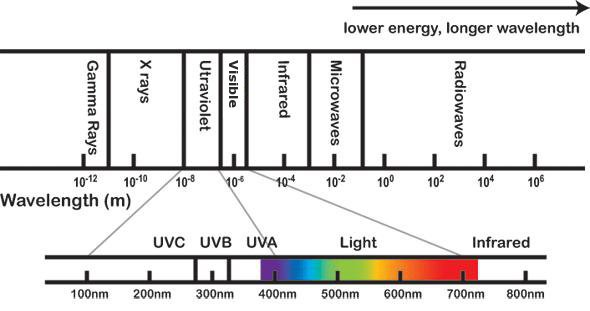
\includegraphics[width=0.4\textwidth]{EMRSpectrum.jpg}
\end{wrapfigure}
There are three types of UV rays: UVA, UVB, and UVC, each with a respective wavelength range and energy, which determines the harm that each of them can cause. UV radiation (UVR) can cause “DNA damage (formation of cyclobutane pyrimidine dimers), gene mutations, immunosuppression, oxidative stress, and inflammatory responses.” \cite{fox_review_2010} UVR can cause many different kinds of DNA damage, for example: if UVR can mutate the p53 tumor suppressor gene, it could cause skin cancer, as cell mitosis is no longer being regulated. The p53 tumor suppressor gene regulates cell division and keeps cells from growing and dividing too fast or if the cell has an issue. It makes sure everything is needed for cell division and everything is correct before fully creating a second cell. If something is wrong, the cell goes into apoptosis, which is the death of a cell as a means of preventing the mutation from spreading.

UVC has the shortest wavelengths, consisting of only 100-280 nm. Since energy is inversely proportional to wavelength, this means that UVC has the highest energy of all three types of UVR. UVC is completely absorbed by the Earth’s ozone layer and is unable to reach the Earth’s surface. Luckily, this means that we will not need to worry about UVC in this experiment as it is unable to reach humans in the first place.


UVB has the second highest energy, with wavelengths of 280-315nm. UVB makes up about 1-10\% of all UV that reaches the earth’s surface, as the ozone layer also filters it. Because of its shorter wavelengths and higher energy, it can penetrate the upper layers of the epidermis. While it can help the skin produce vitamin D3, it is also able to cause DNA damage, forcing cells into apoptosis. When DNA is damaged by UVB light, it triggers photochemical reactions between the bases of the DNA. 75\% of this damage is attributed to the cyclobutane pyrimidine dimers, which occur when 2 adjacent pyrimidine bases, such as cytosine and thymine, bond together. \cite{noauthor_cyclobutane_2020} This rapid apoptosis means that cells are dying off quickly, which is what we call a sunburn. In severe sunburns, blistering can occur. UVB also causes serious skin cancer called melanoma. It is a thousand times more effective at causing sunburns than UVA.

\begin{wrapfigure}{l}{0.4\textwidth}
  \centering
  \caption{Cyclobutane Pyrimidine Dimers \cite{noauthor_cyclobutane_2020}}
  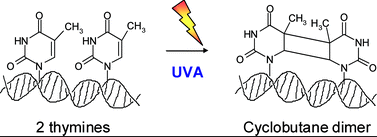
\includegraphics[width=0.4\textwidth]{CPD.png}
\end{wrapfigure}
UVA makes up about 90-99\% of all UV rays that reach the Earth, with wavelengths of 315-400 nm. It is not filtered by the ozone layer like the other types of UVR, as it has longer wavelengths and lower energy. Despite this lower energy, UVA can penetrate deeper into the skin. Because of this, UVA affects not only the epidermis as UVB does, but it also affects the deeper layers, photo-oxidizing melanin and primarily producing free radicals (an unstable molecule that can build up and cause damage to other molecules). Overall, UVA is in greater abundance and is more likely to cause long-term effects like tanning and skin aging, than UVB. Despite this, it does not cause as much damage as UVB. Although it penetrates deeper, it does not damage the cells as much due to its lower energy.

\begin{wrapfigure}{r}{0.4\textwidth}
  \centering
  \caption{The UV Index \cite{us_epa_uv_2015}}
  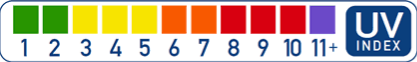
\includegraphics[width=0.4\textwidth]{UVIndex.png}
\end{wrapfigure}
The UV Index measures the UV radiation level on a scale from 1-11+. It is typically calculated with this equation: $Erythemal radiation [W/m^2] X 40m^2/W = UV Index$. This equation is typically used to calculate the average UV index throughout the day, so it accounts for weather, specifically clouds. Since we are only measuring the amount of UV that can pass through the sunscreen, we are directly measuring voltage, which is proportional to the UV index, but shows how much is being filtered more precisely.

\subsubsection{The UV Sensor}
\begin{wrapfigure}{r}{0.4\textwidth}
  \centering
  \caption{The UV Sensor}
  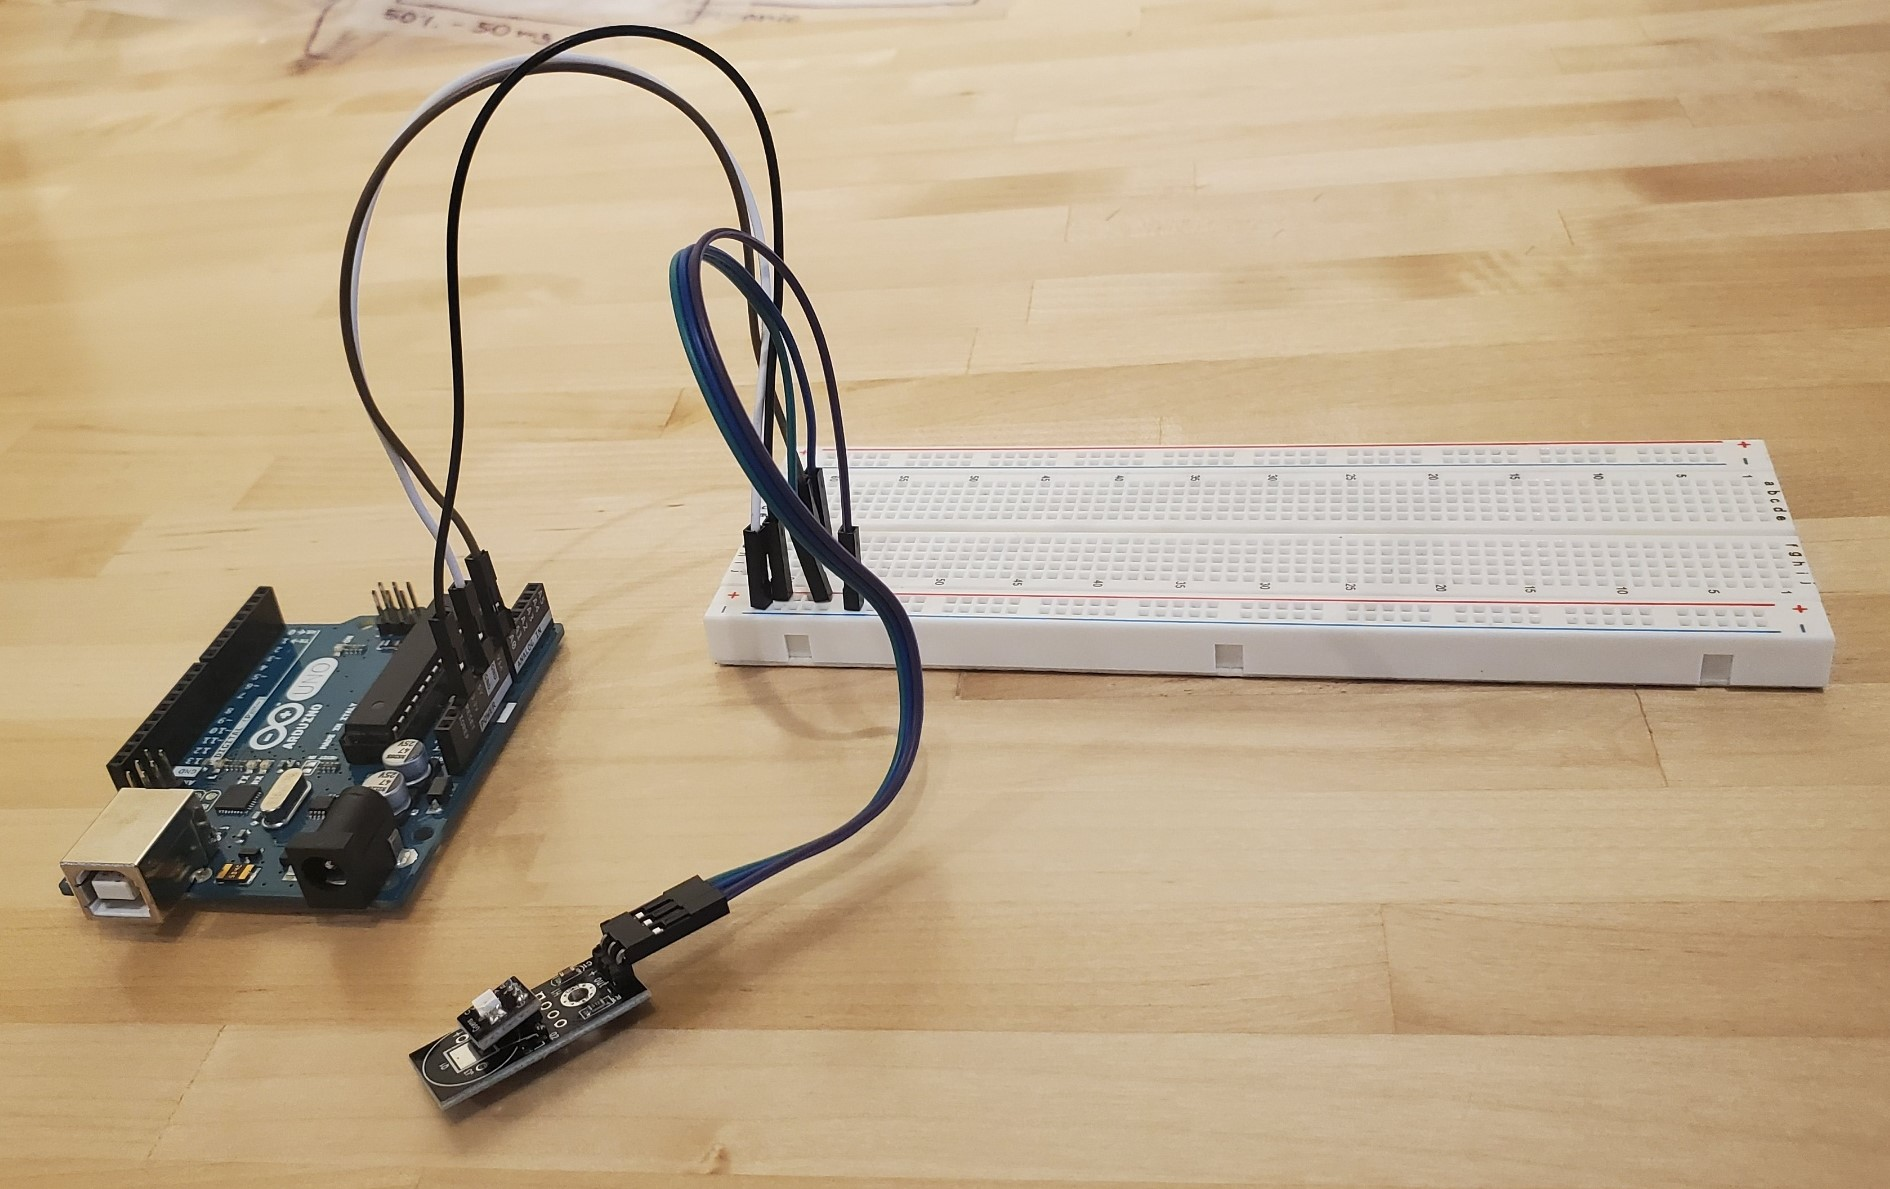
\includegraphics[width=0.4\textwidth]{UVSensor.jpg}
\end{wrapfigure}
We created this sensor in order to determine how much UV light was being filtered by the sunscreens. The sensor takes in UV light, which is able to generate a current. This occurs because the light strikes the anode and gives the electrons enough energy to travel to the cathode. This transfer of electrons generates a current, which is stronger when more photons are actively hitting the photodiode. The Arduino then allows us to read the voltage produced by this current, which then is converted by the code to millivolts and recorded. These millivolts allow us to see a more precise measurement, as the UV index is fairly broad in comparison. To make the sensor, please see section 5: Materials and Methods. 

\subsection{Why Sunscreen Works}
\begin{wrapfigure}{r}{0.4\textwidth}
  \centering
  \caption{Absorption and Emission \cite{noauthor_light_nodate}}
  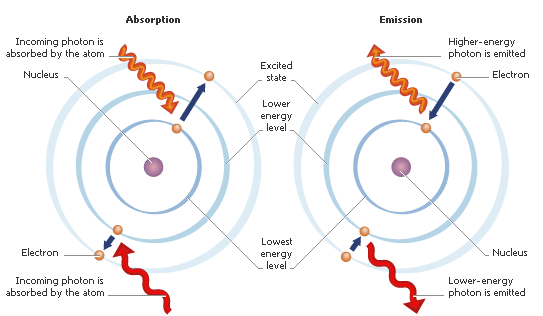
\includegraphics[width=0.4\textwidth]{Absorption.png}
\end{wrapfigure}
As UV light comes into contact with a molecule, the molecule may be able to absorb the ray. This means that when a photon hits an electron, the electron absorbs the photon’s energy, and it jumps to an excited state. Only certain electron jumps can absorb UV light, so the molecule must contain pi bonds or non-bonding orbitals to absorb this spectrum. This is because only a limited number of possible electron jumps can absorb UV light. Different electron jumps require different amounts of energy, which means an electron will only absorb a certain photon if the amount of energy is just right for making an energy jump. The photon allows some molecules, such as oxybenzone to overcome the activation energy and undergo a chemical reaction; however, as the electron relaxes, the molecule goes back to the state which took lower energy. Eventually, the electron releases the energy and returns to its respective orbital, in the ground state. This relaxation of the electron will release the energy as heat, emitting it in the infrared spectrum (700-1000 nm). 

Sometimes, the oscillating electric field of the UV ray will induce an electron, and its electric field,  to oscillate at the same frequency as the incident light. The electron will then emit electromagnetic (infrared) waves in all directions. The ones that are backward in comparison to the incident ray are reflected. Those that are forward in comparison are refracted, meaning their path shifts through the material.

Sunscreens are commonly divided into “chemical” and “physical” labels, with “chemical” sunscreens absorbing UV rays and “physical” sunscreens reflecting or blocking UV rays. These labels and divisions are not necessarily accurate, however, as “physical” sunscreens, while reflective, absorb more UV rays than they reflect. The more accurate labels are “organic” and “inorganic/mineral.” This is because the main separation is that the “organic” sunscreens have carbon-hydrogen covalent bonds while “inorganic”/”mineral” sunscreens do not and are typically transition metals. “Mineral” sunscreens are insoluble chemicals like zinc oxide and titanium dioxide. They provide both UVA and UVB protection and are typically used in the nano form as they provide less of a white cast in this form. “Organic” sunscreens, on the other hand, are soluble chemicals such as oxybenzone, avobenzone, homosalate, and octinoxate.  They are more effective against UVB rays than UVA.
        
Sunscreens labeled as “broad spectrum” typically refer to their ability to protect from both UVA and UVB proportionally. This is specified, because most sunscreens only protect against UVB, as it is the spectrum of UV that is most likely to cause sunburn (it has the most energy and also, more importantly, reaches the person, unlike UVC). This is because scientists didn’t fully understand the dangers of UVA, so sunscreens did not guard against it; however, over time, sunscreen manufacturers began to incorporate ingredients that did protect against UVA and labeled these sunscreens as “broad spectrum”, but without testing requirements until 2011. Only 39\% of consumers stated that the “broad spectrum” label influenced their decision in their sunscreen purchase, with 79\% stating that sweat and water resistance was more desirable. \cite{caribbean_sol_3_2022}

\subsubsection{Possible Sunscreen Dangers}
The U.S. has only approved 16 active sunscreen ingredients, with only eight commonly used; however, there are some concerns regarding the toxicity and harm of both kinds of sunscreens. Since “mineral” sunscreens cause a heavy white cast, many producers use them in the nano form to appeal to consumers. However, this reduces the ingredient’s protection as well as raises concerns over the skin's ability to absorb nanoparticles, as many are now concerned about the possibility of unwanted particles in the bloodstream. Studies have otherwise shown that nanoparticles are not likely to penetrate the skin and should be safe in sunscreens. \cite{mohammed_noninvasive_2020} “Organic” sunscreens, on the other hand, have been shown to cause bleaching in corals and harm aquatic life; states like Hawai’i have even banned some of these ingredients. The FDA has put concentration restrictions on each of these ingredients (FDA), as all of them have a possibility of being toxic in large concentrations.

\subsubsection{The Sun Protection Factor and Why it is Not Being Used}
SPF is a common measure for the protection a solution provides from the sun, but only regarding sunburn. Officially, it is a formula for determining the number of UVB rays that reach the skin (i.e. SPF 30 = 1/30 rays reach the skin); However, SPF is typically “calculated” by determining how much longer it took a volunteer to burn slightly with the sunscreen on than without the sunscreen. It is not an accurate measure in terms of how much UV is truly blocked. Skin is different, people burn at different rates, and the amount of sunscreen applied all affects the rate at which someone would burn. Because only visible burns are tracked, only UVB rays are considered. For these reasons, we have decided not to rely on SPF as a metric for our research.

\subsubsection{Sun Protection and Concentration}
According to the Beer-Lambert Law, concentration and absorbance are directly proportional: $A = \epsilon bC$, where A = absorbance, $\epsilon$ = molar absorptivity, and C is concentration. Also according to the law, as a substance’s concentration increases, so does the absorbance. Therefore, we would expect that when the concentration of zinc oxide is increased, the absorbance of the material should also increase, meaning more sun protection. Our experiment aims to explore this concept and determine the effect of concentration on absorbance. Along with this, the refractive index of a solution also increases as molar concentration increases. This means that with an increase in concentration, sun protection would also increase as more photons are being blocked.

\subsection{Why Zinc Oxide?}
Zinc oxide has been used for centuries, with its first recorded appearance in an ancient Indian medical literature ‘Charaka Samhita’ which identified the pushpanjan (zinc oxide) as a salve for eyes and open wounds. This literature is thought to date from 500 BC or possibly earlier. Throughout the centuries, zinc oxide has been used as the white pigment in oil paint, photocopying, cosmetics, rubbers, plastics, ceramics, batteries, and so much more. \cite{grabenhofer_inside_2022} So why is it used in sunscreen and why are we using it for this experiment?

\begin{wrapfigure}{r}{0.4\textwidth}
  \centering
  \caption{Band Gap \cite{noauthor_semiconductor_nodate}}
  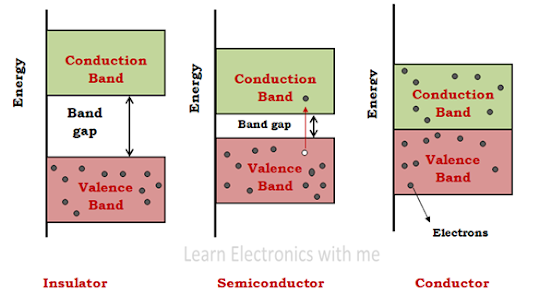
\includegraphics[width=0.4\textwidth]{bandgap.png}
\end{wrapfigure}
The band gap of a molecule (or the energy gap) refers to the energy difference between the valence band and the conduction band. This represents the amount of energy that is required to excite an electron up to a state in which it can participate in conduction, as seen in Figure 7. As a semiconductor, ZnO has a band gap that appropriately corresponds to UVA wavelengths, meaning that this molecule can interact directly with the specific wavelength of UVA light. Zinc oxide in particular has a bandgap of 3.4eV and the range of photon energy for UVA and UVB is 3.10-4.43eV, meaning that zinc oxide can absorb a great amount of photons. ZnO also has a high refractive index (n = 20) as well as an ability to reflect, which means it can scatter many rays. This is why ZnO appears white as a non-nano molecule in sunscreen.


\section{Materials and Methods}
In order to make the UV sensor, the Arduino Uno and the UV sensor had to be connected through a breadboard. This was done by: Connecting the Arduino Uno’s GND to the breadboard’s (-) Pin, the Arduino’s 3.3C to the (+) Pin next to the (-) Pin, and the Arduino’s A0 to the 58h pin on the breadboard. The UV sensor is then added by: Connecting the UV sensor’s Out Pin to the 58j pin on the breadboard, the UV sensor’s (-) Pin to a (-) Pin on the breadboard, and the UV sensor’s (+) Pin to the breadboard’s (+) Pin next to the previous (-) Pin. In total, this uses 6 wires. The code is then uploaded onto the sensor.

First, the varying concentrations of the homemade zinc oxide sunscreen must be formulated. This is done by adding the required amount of zinc oxide to a plastic bowl, then adding the required amount of lotion and mixing thoroughly. Set aside and repeat for the next concentration. The table below provides values for concentrations 0\%-50\%, yielding 14g of sunscreen.
\begin{center}
\begin{tabular}{ | m{9em} | m{7em} | m{5em} | }
    \hline
    Concentration (\%)& Zinc Oxide (g)& Lotion (g) \\
    \hline
    0 & 0 & 14 \\
    \hline
    5 & 0.7 & 13.3 \\
    \hline
    10 & 1.4 & 12.6 \\
    \hline
    12 & 1.7 & 12.3 \\
    \hline
    15 & 2.1 & 12.0 \\
    \hline
    20 & 2.8 & 11.2 \\
    \hline
    25 & 3.5 & 10.5 \\
    \hline
    50 & 7 & 7 \\
    \hline
\end{tabular}
\end{center}
\begin{wrapfigure}{r}{0.4\textwidth}
  \centering
  \caption{The Sunscreens}
  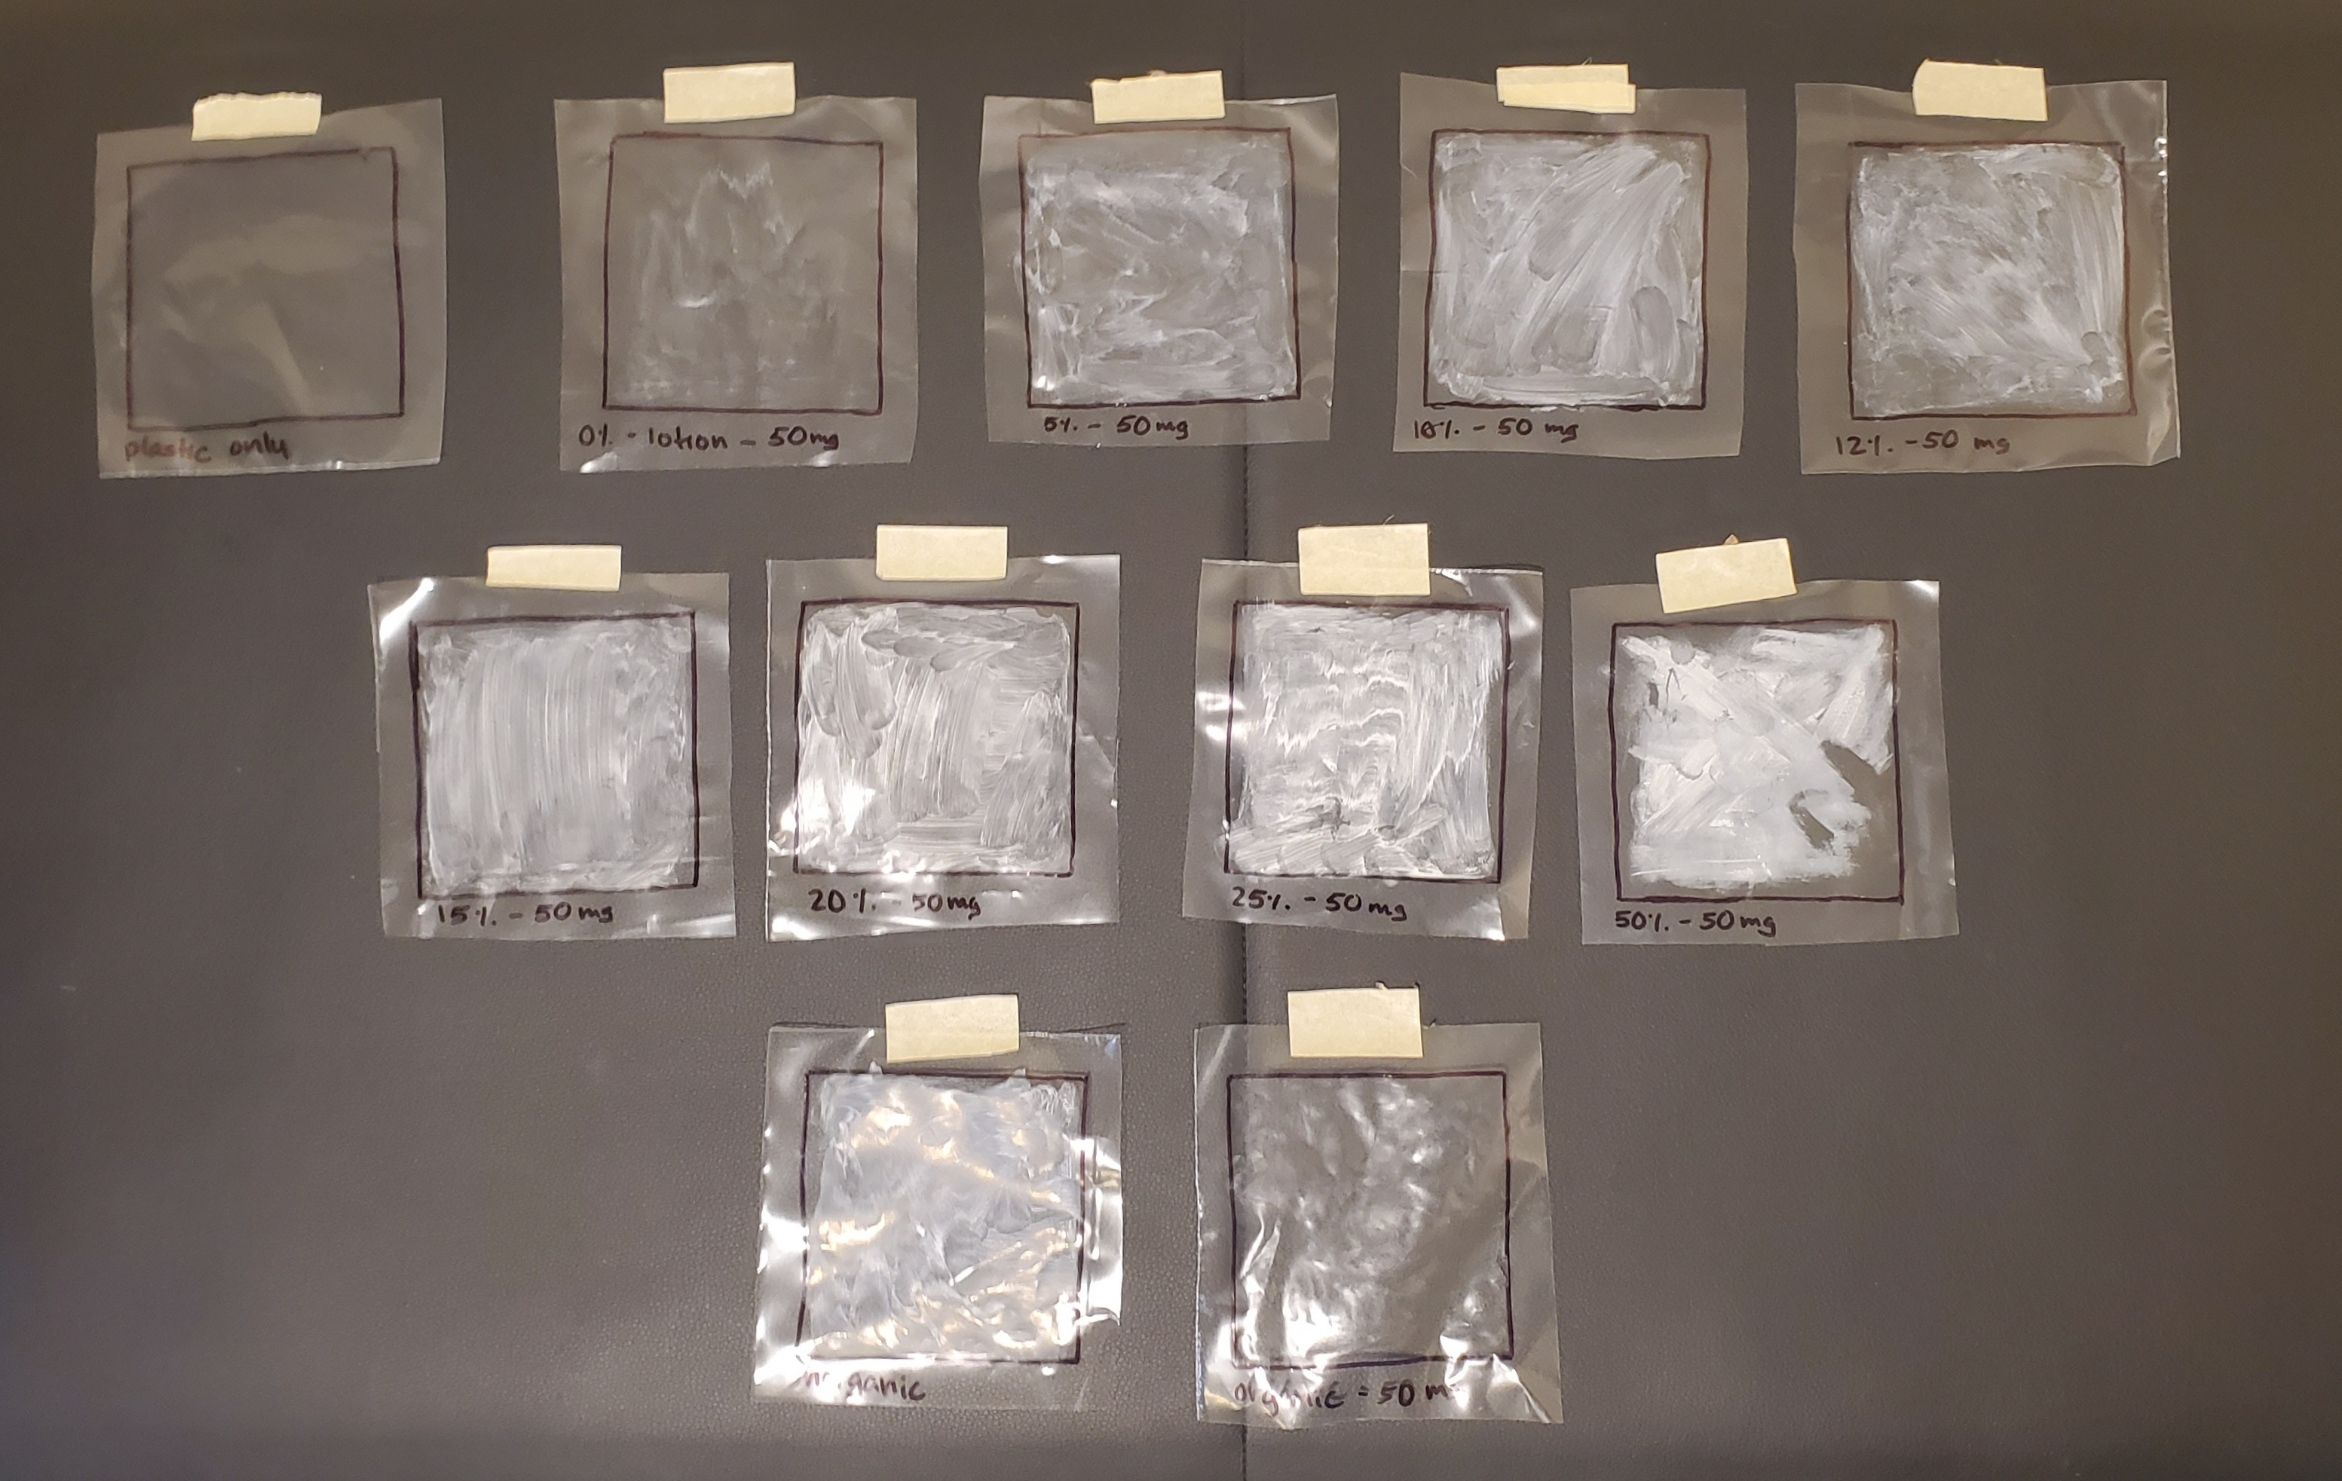
\includegraphics[width=0.4\textwidth]{Sunscreens.jpg}
\end{wrapfigure}
We then cut out 11 plastic squares, drew 4 in by 4 in squares on them using a black sharpie and labeled each one: Plastic, 0\% zinc oxide, 5\% zinc oxide, 10\% zinc oxide, 12\% zinc oxide, 15\% zinc oxide, 20\% zinc oxide, 25\% zinc oxide, 50\% zinc oxide, Banana Boat (Organic), and Cetaphil (Inorganic). 50mg of each sunscreen was weighed out and spread evenly across its respective square (keeping inside the black lines), with “Plastic” being left empty. The use of an empty plastic square and a 0\% concentration (only lotion) square in order to see how much UV is absorbed by each. This is because we knew that both plastic and lotion have a tendency to absorb small amounts of UVR. Although this is not a significant amount, it still shows that they both have a small impact on testing the sunscreens.

To conduct the experiment, all equipment was taken outside. A base reading was recorded before testing the “Plastic” square. 4 readings were then taken under the “Plastic” square, with each reading being taken at a different spot on the square. This procedure was then done with each sample, from base reading to 4 readings. 

\subsection{Experimental Design}
In the beginning, we tested plastic, 0\%, 10\%, 15\%, 20\%, 25\%, and 50\% using 200mg on each square. This was done in order to get an easier spread; however, after the experiment was conducted, we realized that we wanted more data points and decided to test 5\% and 12\% in our next trial. We also noticed that 200mg was not a realistic amount of sunscreen, as people do not typically apply 200mg per each $16 in^2$. Rather, sunscreen is typically tested at $2 mg/cm^2$ \cite{fung_spfs_nodate} and typically worn at $0.5 mg/cm^2$, or $3.25 mg/in^2$. Since each square is $16in^2$, this was adjusted in order to represent a more realistic approach according to this typical application. \cite{taylor_simple_2002} Future experiments were then conducted with 50mg of each sample rather than 200mg.

We then made 5\% and 12\% for our second trial and reran the experiment using 50mg per square. The data showed that both 5\% and 12\% had performed higher than expected. This was attributed to possible degradation in the older sunscreens, as they had been made around 2 days before the others. Each sunscreen was then remade before the third trial. We also noticed during this trial that the spreading was pretty inconsistent, as denser spots blocked more UVR. This made us realize that more data points were needed from each square in order to accommodate for uneven spots.

Finally, we decided on a final design in which all sunscreens were freshly made, tested in 4 different spots to get a more representative average, and conducted on a very sunny day in order to have as much UVR to test with as possible. 

\FloatBarrier
\section{Results}
\begin{figure}
  \centering
  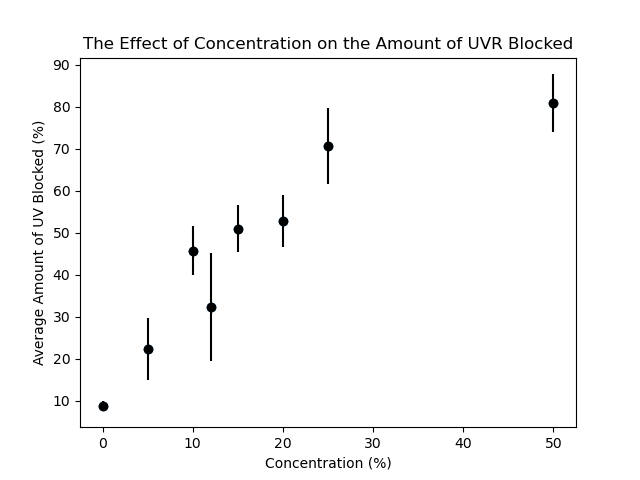
\includegraphics[width=0.5\textwidth]{SunscreenDataPlotZO.png}
  \caption{Scatter plot displaying each sample with a varied concentration of zinc oxide with respect to the amount of UV each sample blocked.}
\end{figure}
\begin{figure}
  \centering
  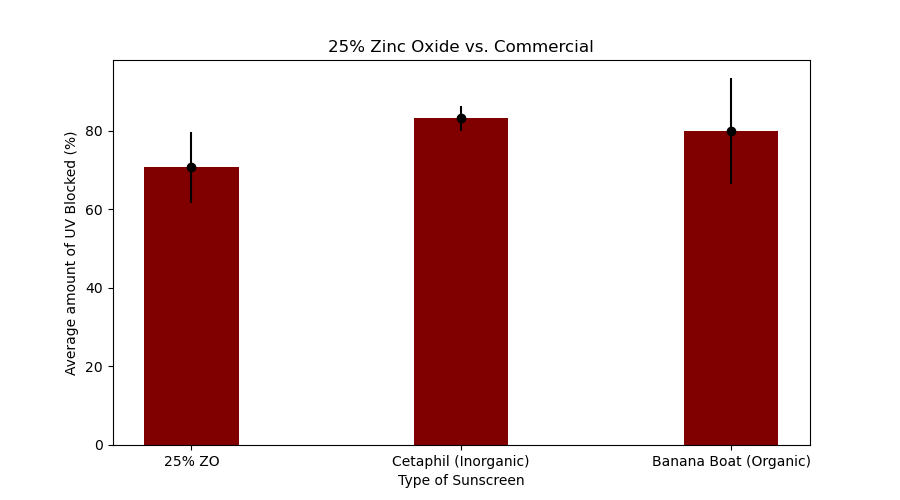
\includegraphics[width=0.55\textwidth]{25ZOvsCommercialPlot.png}
  \caption{A bar graph comparing the two commercial sunscreens to the 25\% zinc oxide.}
\end{figure}
\begin{figure}
  \centering
  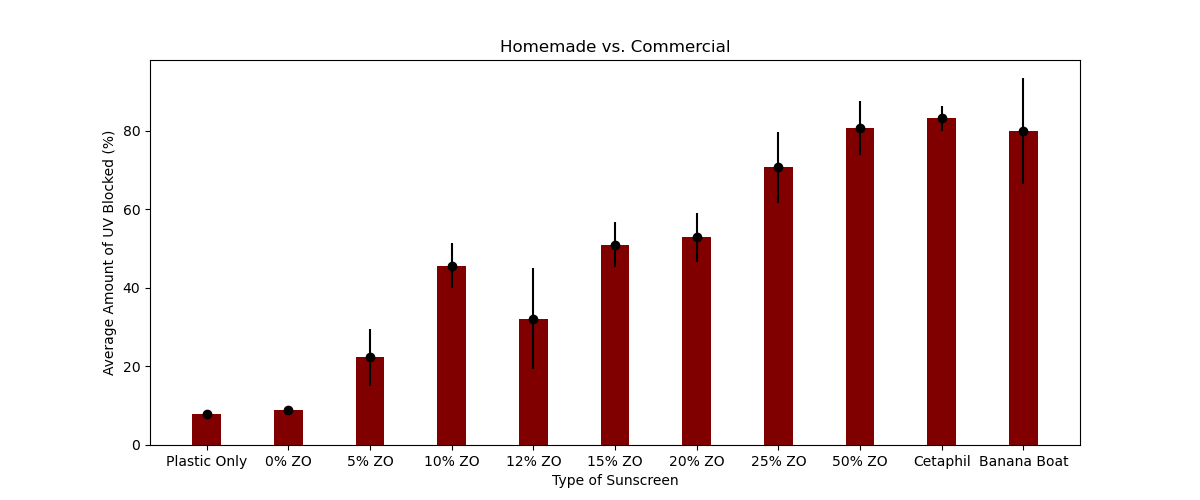
\includegraphics[width=0.65\textwidth]{SunscreenDataPlot.png}
  \caption{A bar graph comparing the two commercial sunscreens, a blank square, and all concentrations of zinc oxide.}
\end{figure}

\section{Discussion}
\begin{wrapfigure}{r}{0.4\textwidth}
  \centering
  \caption{The Beer-Lambert Law \cite{noauthor_beers_nodate}}
  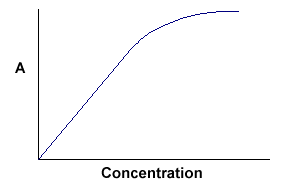
\includegraphics[width=0.4\textwidth]{BLCurve.png}
\end{wrapfigure}
According to Figure 9, as the concentration of zinc oxide increased, the amount of UVR blocked also increased. However, after 25\%, the amount of sun protection seemed to plateau. This positive correlation between concentration and sun protection could be partially attributed to the Beer-Lambert Law, as stated earlier. Since zinc oxide has a higher tendency to absorb rather than reflect, this absorbance must have increased as the concentration increased, providing more sun protection. But why did the graph stray from a linear relationship as concentration goes over 25\%? A possible explanation could be that the Beer-Lambert Law is not obeyed at higher concentrations as higher concentrations tend to have more interactions between solvent and solute that decrease absorbance.

Is homemade sunscreen nearly as effective as commercial sunscreen? According to Figure 10, even over the legal concentration set by the FDA, the homemade zinc oxide sunscreen did not block as much UVR as the commercial sunscreens did. When compared to commercial sunscreens, the 25\% zinc oxide sunscreen, which is the limit set by the FDA, did not perform nearly as well. With only an average of 71\% UV blocked compared to the average of 83\% UV blocked by the inorganic sunscreen and the 80\% blocked by the organic sunscreen, homemade sunscreen is not as protective as commercial sunscreens but could be a considerable alternative for those wary of commercial sunscreens.


\section{Acknowledgments}
I would like to thank my mentor Abigail Wilson for her valued guidance, direction, and comfort. I would also like to thank Rhonda Crespo, Mark Galassi, and my fellow interns at the Institute for Computing in Research for their help and support. I would also like to thank Richard Pitman for writing my recommendation letter, as well as thanks to both Richard Pitman and Derek Buschman for helping to further my interest in the sciences and helping to teach me over the past 3 years.

\subsection{Conflicts of Interest}
The author declares that there is no conflict of interest regarding the publication of this article.

\newpage
\printbibliography

\end{document}
